\documentclass{scrartcl}
% \documentstyle{article}
\usepackage{comment}
\usepackage{amsmath}
\usepackage{caption}
\usepackage{graphicx}
\usepackage{subfig}
\begin{comment}

\end{comment}
\usepackage{xcolor}
\newcommand\todo[1]{\textcolor{red}{#1}}

\DeclareCaptionType{mycapequ}[][List of equations]
\captionsetup[mycapequ]{labelformat=empty}

\providecommand{\comm}[1]{{\bf[ #1 ]}}
\providecommand{\commd}[1]{\comm{D: {#1}}}

\begin{document} 
\title{Master Thesis Working Document}
\subtitle{What can the parameters of IRT based learner models tell us?}
\author{Lieuwe Rekker}
\maketitle
\nocite{labelcombi}
\nocite{lftransfer}
\nocite{importance}
\nocite{knowledgeproblem}
\nocite{modelreview}
\nocite{eirt}
\nocite{pfa}
\nocite{ktpfa}
\nocite{skillcombi}
\nocite{lfa}
\nocite{blackart}
\nocite{hambleton}
\nocite{bridge}
\nocite{ct}
\nocite{algebra}

%\listofmycapequs

\section{Introduction}
\begin{comment}
Many current intelligent tutor systems (ITS) use learner models that can give indications of to what extent a student has mastered a particular skill and even how fast students learn.  The quality of these models is generally measured by how well these models predict 'one question into the future' performance, which is what these algorithms\commd{You didn't mention any algorithms yet, just models - and even then, they maximimize the likelihood of the training data...} are made to maximize. Parameter values from these models are also inspected and stated to represent students' knowledge levels, how fast students learn, how difficult questions are etc. It would thus be wise to inspect other factors beyond the accuracy of the model to gain some idea of under what conditions they actually convey some stable real world factor or are rather part of a more black-box like model that performs well on its prediction task, but whose parameters are otherwise meaningless. \cite{knowledgeproblem} shows that this is indeed a problem: widely differing parameter settings can yield similar, (near) optimal performances. This proposal proposes research to explore if parameters of learner models hold meaning in real life.

The approach of this research is from the perspective that models resemble reality, but are necessarily not precise mirrors of it. Initially generated data is used to see how well parameter values can be retrieved at all and to see what happens to parameters when there is a mismatch between model and 'reality' (i.e. training a model on data generated by a different model). The amount of training data is looked at especially, since even if stable parameter values can be found, this will probably break down at some point. In the case of real data, original parameters and models are unknown. Over multiple training runs on different data-sets, variation in parameter values can be inspected. High variation here indicates that (despite possible good prediction performance of the model as a whole) the parameter does not represent anything in reality.
\end{comment}
\commd{Provide short motivation for ITS's first.} Today more and more intelligent tutor systems (ITS) are being used, both in research settings and in the world at large. An ITS is a computer program used by students to learn about different subjects and generally entails that students solve problems within the system. Data from these systems have been used to build models of how students learn.\commd{Most learner models do that indeed, but some restrict themselves to the probability of a correct answer... We don't like those, but still.} These learner models in turn have been used in ITSs to estimates the level of the student and adjusts the problems it presents to the student accordingly.\commd{Reformulate in terms of possible usuage of student models.} In research these learner models are generally evaluated by looking at some measure of how the performance predicted by the model fits the real data.\commd{Will need some cites. And, I would cute the word real.} In this research a set of learner models based on item response theory (IRT) will be discussed and it will be examined when the parameters that are fit in these models are stable.\commd{Why? motivate please}

In psychology and more notably psychometrics, how students perform on problems has long been a field of research. The activity in this field was hastened by the necessity for standardized testing. This has eventually led to the development of item response theory (IRT) (for a good overview see \cite{hambleton}). In the models stemming from IRT, students are characterized by a skill level and problems are characterized by factors such as difficulty and discrimination. Through decades of research and practical use (especially for standardized tests) IRT has gained a solid theoretical and experimental basis, which makes it a logical basis for use in ITSs in estimating the level of students. Problematic though in the application of this theory to ITS data is that learning is not taken into account.\commd{Alternative, ...is that IRT assumes the compentence of the students to be constant for the duration of the test. In ITS, which are designed to help students learn, this can obviously not be assumed.} Within a test learning is not much of an issue, but in an ITS data is collected over longer time spans and learning is actually meant to occur. \commd{ from here onwards the structure is a bit illogical. First cluster all information you want to give about IRT by itself first, then mention why you want to extend, then mention the how, then the problems that one can encounter by doing so, that a comprehensive evaluation and comparison of these models has not yet been made - and then state what your research will be, (and maybe mention the use of your research for educators and researchers)} Therefore the adaptations of IRT models used on this kind of data incorporates a learning rate.

In IRT there are established methods to see if obtained parameters are significant as well as methods that check whether its assumptions are met. This gives confidence that found parameters for students and problems are meaningful and can be used to make statements about student skill and item difficulty. In the case of the models used for ITSs, generally only model fit compared to the data (in various forms, most notably one-step-ahead prediction accuracy) is taken into account. There are some exceptions where concerns are raised on the plausibility of parameters \cite{ktpfa}, \cite{knowledgeproblem} and accuracy of parameters \cite{blackart}. Not looking further into the accuracy of these parameter estimates is at the least a missed opportunity (e.g. knowing how easy certain skills are to learn, how difficult certain items are, or how fast a particular student learns can be valuable information, even if simply to improve the ITS) and might already be used wrongly in some cases (for example making statements on the difficulty of questions, without knowing whether the fitted values can be trusted).

This research will look at the influence of how certain factors influence the accuracy of parameters estimation. When applying IRT to test results, generally no external measure is used to check the found difficulty and skill parameters against, rather internal validity is used to see if the assumptions of IRT hold \cite{hambleton}. For example, when estimating the difficulty of an item, it should not matter whether the results of low or high ability students are used to estimate the difficulty. If this is not the case, this indicates that some assumptions are not met and makes the parameter values found of questionable value. This research will take a similar approach in looking at the found parameters. The research will be split into two parts. In the first part generated data is used, so that the real parameter values are known and effects of different factors can be estimated. In the second part real data will be cut into pieces so that variance of parameters can be determined. In combination with the first part of the research it is hoped that conclusions can be drawn as to whether the parameter values found are useful and whether the data-fit measures normally looked at provide some clue to this usefulness.

\section{Models}

\subsection{IRT Models}
For every question asked an IRT model uses the student $s$ and the item $i$ as input and return a probability $P$ that the question is answered correctly. The function at the basis of providing this probability is the logistic ogive function (\ref{eq:logistic}). Each student has exactly one parameter associated with them which represents the ability of the student and is here named skill and indicated by $\theta$. This parameter is generally the parameter of highest interest in tests as it can be used to order the level of skill of the different students. The number of parameters associated with items and how all these are combined into $x$ differs per particular model and is discussed in the following paragraphs.
\begin{equation}
\label{eq:logistic}
\sigma(x) = \frac{1}{1+e^{-x}}
\end{equation}

The 1PL model, also known as the Rasch model has one parameter ($b$) per item (hence the name), which stands for the difficulty of the item. The entire formula for a questions probability of a correct answer is then: $P = \sigma(\theta_{s} - b_{i})$. This means that when the skill of the student and the difficulty of the item are on a par, the student has a probability of .5 to answer the question correctly. Note that one can keep the same model while changing the parameter values by increasing or decreasing all $\theta$ and $b$ by the same amount.

The 2PL model expands the 1PL model with the parameter $a$ which is called the discrimation of the item. The 2PL then looks like this: $P = \sigma(a_{i} (\theta_{s} - b_{i}))$ The term discrimination comes from the fact that a high discrimination causes $P$ to change quickly when $(\theta_{s} - b_{i}))$ is small and thus the performance of students who are close in skill can be more easily distinguished. The flip-side here is that when $(\theta_{s} - b_{i}))$ isn\'t small, $P$ will more quickly drop to 0 or rise to 1, concealing any difference between student skill at those levels. 

The final IRT model discussed here is the 3PL model which adds a chance parameter $c$. This model takes into account that on occasion the student could answer a question correctly by taking a (educated) guess. This phenomenon is of course most prevalent in multiple choice tests where the chances of correctly guessing the answer are relatively high. The model effectively changes the lowest probability to the level of $c$. In this thesis this model is left out of consideration as none of the learning models are based on it and none of the data is multiple choice.

All models used in this research are based on item response theory and use a version the 2 parameter item response function (IRF) \commd{No they don't, the first couple you mention use the 1 parameter IRT, also called Rasch, model}. The basis of this function is the logistic ogive function \ref{eq:logistic}. The most basic 2 parameter IRF is shown in \ref{eq:irt}. Here i stands for item and s stands for student. $\alpha$ is the discriminatory power of the item i.e. how much knowledge matters in how well a student does on that item. $\beta$ is the difficulty of the item i.e. how high a students skill should be to achieve a P of .5. $\theta$ is the skill of a student, indicating how well the student has mastered a knowledge component. The value of the function is interpreted as the probability that the student answers a question correctly. This is the same interpretation that is used throughout all models in this research.



\begin{equation}
\label{eq:irt}
P = \sigma(\alpha_{i} (\theta_{s} - \beta_{i}))
\end{equation}

All models used in this research employ an important extension: it incorporates learning by students. Skill, $\theta$ is split up into an initial part and a learning rate, so that each time a question is answered the skill of the student increases. In the ITS there are many different knowledge components and thus the parameters are fit per knowledge component. Depending on the data-set used an item can have multiple components associated with them, creating the necessity to combine multiple item response functions.

\todo{Say something about the fitting procedure for each seperate model.}\commd{what, here? or do you mean the alternate ML optimization of student and item parameters? }

\commd{List the assumptions each model makes. Either in each subsection, or in a separate subsection}

\subsection{Learning Factor Analysis (LFA)}
\label{sec:LFA}


LFA uses a simplified version of the IRF, but extents it by introducing a learning rate as discussed in the introduction and by allowing multiple knowledge components to be associated with a single item. The combination of KCs is made by summing the learned part of knowledge and the difficulty of the KC for every KC that is linked to the item.

\begin{equation}
\label{eq:afm}
P = \sigma(\theta_{s,0} + \sum_{c \in KC}  \eta_{c} t_{s,c} - \beta_{c})
\end{equation}
\commd{So the start competence is the same for every knowledge component/skill, but the learning speed can vary per KC/skill... that is an assumption that is explicitly rejected in the eIRT paper.}

The simplification of the model is done by dropping $\alpha$ (this model is called the Rasch model). The splitting of $\theta$ leads to the introduction of an initial skill $\theta_{0}$ defined per student, a learning rate $\eta$ defined per KC (i.e. the KC determines how fast or slow learning occurs) and a number of times that a student has seen items belonging to this particular knowledge component $t_{s,c}$. Please note that in the the original LFA $\beta$ is added. It is subtracted here to maintain similarity to the original IRF and ensure uniformity with the other models used. This has no other effect than that the signs for $\beta$ are reversed.

When looking at a data set where only a single knowledge component is linked to every item, $\beta$ and $\theta_{0}$ are not independent: we can raise both by any amount. To solve this issue, the average value of $\theta_{0}$ is set to 0.
\subsubsection{Combining knowledge components}
\label{sec:comb}
Something more can be said about the way KCs are combined. In \cite{skillcombi} Cen et al. show that in practice there is no difference in performance between an additive model (as used here) or a conjunctive model (where probabilities of individual KCs are multiplied). Nevertheless the authors already mention that this is probably the case because for most KCs $\beta < \eta_{c} t_{s,c}$, meaning that adding KCs does decrease the chance of answering the question correctly as would be expected. In their paper they already propose using a data set where ($\beta > \eta_{c} t_{s,c}$) to see if this is indeed why this way of combining KCs works well in practice.

The experiment proposed above is put to the test here. Fitting a conjunctive model is hard in practice, but generating data using one is rather straightforward. Whether a real life data set contains many questions where skills are such that $\beta < \eta_{c} t_{s,c}$ cannot be said at this point. Even if this is not the case though, it can be argued that the parameter values can be skewed slightly to ensure that this occurs. The rationale behind is, is that the fitted values obtained from the real data may be skewed towards $\beta < \eta_{c} t_{s,c}$ due to a additive model being used in the fitting process. It would then be expected though that the retrieved parameters using these values would be skewed towards $\beta < \eta_{c} t_{s,c}$ again.

\subsection{Performance Factor Analysis (PFA)}
PFA is a direct extension of LFA. In PFA separate learning rates are used for questions answered correctly and questions answered incorrectly. Additionally $\theta_{0}$ is dropped. As put forward in \cite{pfa} $\theta_{0}$ is dropped because this extension is made mostly to make this model more useful in ITSs. Leaving out any student specific parameter makes the model more easily applicable to students not used in the fitting procedure. As noted in both \cite{ktpfa} and \cite{blackart}, leaving out $\theta_{s,0}$ makes parameter estimates worse. Since prediction for students who were not part of the fitting procedure is not a primary concern here, a model that does include $\theta_{s,0}$ (as done in \cite{ktpfa} and \cite{blackart}) is used instead of PFA and will be referred to as PFA+.

\begin{equation}
\label{eq:pfa}
P = \sigma(\theta_{s,0} \sum_{c \in KC}  \gamma_{c} g_{s,c} + \rho_{c} f_{s,c} - \beta_{c})
\end{equation}
\commd{Is there a minus sign missing here? same assumption as the last, but two different learning rates. }

Here $\gamma$ is the learning rate of the KC for correct answers and g is the number of questions answered correctly. Consequently $\rho$ is the learning rate of the KC for incorrect answers and f is the number of questions answered incorrectly. Just as with LFA above the sign for $\beta$ was reversed compared to the original.

\begin{comment}
To compare the PFA parameter values to LFA values, the weighted average (according to the ratio g:f for each problem) of $\gamma$ and $\rho$ should be compared to $\eta$. $\theta$ cannot be compared when comparing PFA on LFA data, vice versa, $\theta$ should be compared to 0. In case of PFA+ $\theta$ values can be compared directly.

\begin{mycapequ}
\begin{equation}
\eta_{c}: \frac{\gamma_{c} g_{c} + \rho_{c} f_{c}}{g_{c}+f_{c}}
\end{equation}
\caption{Comparison of LFA parameters to PFA parameters}
\end{mycapequ}
\end{comment}

\subsection{extended Item Response Theory (eIRT)}
\label{sec:eirt}
The extended Item Response Theory model by Roijers et al \cite{eirt} is the most straightforward extension to the standard IRT model.

\begin{equation}
\label{eq:eirt}
P = \sigma(\alpha_{c} (\theta_{s,0} + \eta_{s} t_{s,c} - \beta_{c}))
\end{equation}
\commd{Only one competence and learning speed.}

Similar to LFA $\theta$ is replaced by initial skill and a learning rate. Here the learning rate is taken per student though rather than per knowledge component as is done in LFA and PFA. With $\theta$ split up, it would seem that $\alpha$ obtains a slightly different meaning. For $\theta_{0}$ it still has the same discriminatory function. When looking at $\eta$ though, $\alpha$ directly impacts it as a modifier, making learning easier (>1) or more difficult (<1).

\todo{Actually I have no clue on the correct mathematical vernacular, so please nudge me to the right terms to make this more understandable/consice}
It should be noted that different parameter settings can lead to exactly the same model. E.g. all $\theta$s and $\beta$s could be increased by the same amount and the model would still be the same. To still be able to compare parameter values and variances the parameters should be normalized as follows. The average of $\theta{s,0}$ will be set to zero as to resolve the dependency with $\beta$ values. The standard deviation of $\theta$ will be set to 1 as to fix the dependency between $\alpha$ and the other parameters.

\subsubsection{Adapting eIRT}
eIRT as defined by Roijers et al does not incorporate multiple skill steps. In order to be trained on multi-skill data and to be similar to the other models \ref{eq:sumeirt} will be used as a multi-skill extension of the eIRF. To distinguish this version from the original eIRT, this extended version will be denoted as seIRT. A notable difference here is that $\theta_{s,0}$ is divided by the number of KCs involved. This is because $\theta_{s,0}$ should only be added once just as in LFA/PFA, but nevertheless it should be modified by the corresponding $\alpha_{c}$s as well.

\begin{equation}
\label{eq:sumeirt}
P = \sigma(\sum_{c \in KC} \alpha_{c}(\frac{\theta_{s,0}}{|KC|} + \eta_{s} t_{s,c} - \beta_{c}))
\end{equation}

Please note that in the multidimensional case the dependency between $\theta{s,0}$ and $\beta$ is most likely no longer there. The dependency between $\alpha$ and the other parameters still exists though and should still be resolved by fixing the standard deviation of $\theta_{s,0}$ to 1.

\begin{comment}
In comparing seIRT's (or eIRT's) parameter values to those of LFA $\beta$ should be multiplied by $\alpha$. $\theta$ is to be multiplied by a weighted average of $\alpha$ (according to the ratio of KCs of the questions that the corresponding student has answered). Finally a weighted average of $\eta$ per KC should be taken according to the ratio of questions each student has answered containing that KC. seIRT can be compared to PFA by combining the steps above with the steps needed to compare PFA to LFA.

\commd{Let's discuss this: $\eta_s$ is constant per student, and alpha should be inside the sum if you want ot avg it. }


\begin{mycapequ}[!ht]
\begin{equation}
\begin{aligned}
    \beta_{c}:  &  \alpha_{c}*\beta_{c} \\
    \eta_{c}:  &  \alpha_{c}*\frac{\sum_{s \in S} \eta_{s}*t_{s,c}} {|t_{c}|} \\
    \theta_{s,0}: & \theta_{s,0}*\frac {\sum_{c \in KC} \alpha_{c}*t_{s,c}} {|t_{s}|}
\end{aligned}
\end{equation}
\caption{Comparison of LFA parameters to seIRT parameters}
\end{mycapequ}
\end{comment}

\subsection{Combined Model}
The three models introduced above can all be encompassed by a more complex model.

\begin{equation}
P = \sigma(\sum_{c \in KC}\frac{\alpha_c \theta_{s,0}}{|KC|}+\eta_{s} \gamma_{c} g_{s,c} + \eta_{s}\rho_{c} f_{s,c} - \beta_{c})
\end{equation}

LFA can be obtained from this model by taking $\alpha=1$, $\eta=1$ and $\gamma=\rho$. PFA can be obtained from this model by taking $\alpha=1$, $\eta=1$ and $\theta_{0}=0$ (minus the last one for PFA+). The adapted eIRF can be obtained by taking $\gamma=\rho=\alpha$ and realizing that $\beta$ already incorporates $\alpha$.

\begin{comment}
\begin{mycapequ}
\begin{equation}
\begin{aligned}
    \gamma_{c}:  & \gamma_{c}*\frac{\sum_{s \in S} \eta_{s}*g_{s,c}} {|g_{c}|} \\
    \rho_{c}:  & \rho_{c}*\frac{\sum_{s \in S} \eta_{s}*f_{s,c}} {|f_{c}|} \\
    \theta_{s,0}: & \theta_{s,0}*\frac {\sum_{c \in KC} \alpha_{c}*t_{s,c}} {|t_{s}|}
\end{aligned}
\end{equation}
\caption{Comparison of PFA parameters to full model parameters}
\end{mycapequ}

\begin{mycapequ}
\begin{equation}
\begin{aligned}
    \eta_{s}: \eta_{s}* \frac{\sum_{c \in KC} \frac{\gamma_{c} g_{c} +  f_{c}}{\alpha_{c}}}{g_{c}+f_{c}} \\
    \beta_{c}:  & \rho_{c}*\frac{\sum_{s \in S} \eta_{s}*f_{s,c}} {|f_{c}|}
\end{aligned}
\end{equation}
\caption{Comparison of seIRT parameters to full model parameters}
\end{mycapequ}
\end{comment}


\section{Related work}
\label{sec:RW}
\commd{Right now, this section is a laundry list: it could be improved by adding some more structure.}

In \cite{knowledgeproblem} Beck goes beyond investigating the accuracy of a model (knowledge tracing in this case) and also looks at the parameter values. The authors prime reason for concern lies in identifiability: the fact that widely differing parameter settings can lead to almost identical model outcomes. Although this paper does concern itself with the 'plausability' of parameter values it only goes so far as to nudge the parameter to values deemed plausible rather than asking the more fundamental question of whether the parameter values are useful at all.

Learning factor analysis (LFA) \cite{lfa} is a cognitive model of how students learn. It is a Rasch model\commd{is one of the IRT variants... (you have not mentioned that yet)} extended with a learning rate to model learning over time. In \cite{lfa} LFA is used in the context of a greater cognitive model of learning and skill that includes what knowledge components are linked to what items. The quality of fit (measured as the log likelihood of the entire data set given the model plus some penalty for the number of parameters) is used as a measure of quality of a specific linkage of knowledge components to items.

Performance factor analysis (PFA) is a further extension to LFA. It is introduced in \cite{pfa} as an alternative to knowledge tracing and focuses more on correctly estimating whether a student has mastered a particular knowledge component. The difference with LFA is that learning rate is dependant on whether a question is answered correctly or not. Furthermore initial student knowledge is dropped. The foremost reason for doing so is to make this model work for students of whom no data had been taken into account when fitting the model.

In \cite{ktpfa} Gong et al. also made a comparison between various knowledge tracing approaches and PFA. Whether PFA or KT performs better remains inconclusive. Upon inspecting parameter values they found that many learning rates were negative, which seemed implausible in real life. They noted that upon placing a lower bound of 0 on the learning rate, performance improved.  Additionally the authors used a pretest and correlated the performance on this test to the initial knowledge parameter from the model. In this set-up an adapted version of PFA (the same version that will be used in this research: the original doesn't use initial student knowledge) showed the highest correlation).

In \cite{blackart} Yudelson et al. show some particular factors that can negatively influence the quality of PFA models. One of the factors looked at here is model complexity: on the one hand this is done by using a more finegrained set of KCs and on the other hand by adding another parameter to the PFA model. In evaluating their results the authors did not only look at accuracy measures, but also inspected values for specific parameters. \todo{how did they get their standard deviations for the parameters? They don't seem to have split their data?} In inspecting learning parameters they also noted how the learning parameter for wrongly answered questions are often negative when initial knowledge is not included in the model. They concluded that PFA not so much models student learning in this case, but rather performs some kind of 'error tracking' in order to produce good estimates of skill despite not having any additional information on the student. They therefore prefer an adaptation of PFA that includes initial student knowledge.

In \cite{eirt} Roijers et al. extend the 2PL IRT function to include a learning rate. This new version is called extended IRT (eIRT). There are two important differences in how this model has been extended and how LFA and PFA came to be. First LFA and PFA use a multidimensional model, which means that multiple skills can be associated with a single problem. Moreover in eIRT the learning rate depends on students, while in LFA and PFA the learning rates depend on the skills. Roijers et al. perform experiments using generated data, that shows that parameters can often be retrieved from the data. Additionally they have a real life data-set based on 14 students from three different groups. With the small amount of data in their real life set, they conclude based on their previous experiment that only rule difficulty and student initial knowledge can be determined with enough accuracy. After training the model on the data the fitted initial knowledge of the three different groups confirmed their hypothesis of the ordering of average initial knowledge per group. Also the ordering of difficulty of the rules involved is indistinguishable to rankings made by experts. The authors thus showed that the difficulty and initial knowledge parameters obtained reflect the ordering of these in real life.


\section{Research Question}
\label{sec:RQ}
The main question looked into in this thesis is "When are parameter values found in fitting IRT based models distinguishable?". The interpretation of this question is specified in this section and some subquestions are defined which provide structure for the conducted experiments and the discussion of the results. The questions are each formulated in a subsection and referred to throughout the rest of this thesis.

Distinguishable here refers to the need of knowing if the values of parameters are distinct rather than knowing how reliable any particular value is. I.e. the important question would be 'If the value for Tim's initial knowledge is higher than John's is this actually correct?' Thus instead of looking at how reliable particular values obtained in fitting the model are, it is looked at how reliable the ordering of the different values are.

%Distinguishable will not have a clear distinguishable or not answer, but will rather have
There are different levels on which distinguishable can be looked at. In the question above it is on the level of two specific parameters. The default level on which this question will be answered is on the level of parameter type: how well are all the parameters of a particular type distinguishable from each other (macro level). Nevertheless some energy is put into exploring this question on the micro level: i.e. can we say something about how distinguishable a specific parameter is from other parameters?

When on the one hand refers to the fact that distinguishable will depend on some factors, such as how much and what data is used in fitting the model. When also refers to finding conditions that indicate how distinguishable the parameters are. In later sections it is seen that finding the distinguishability of parameters is complex, time consuming and restricted to subsets of the data. Thus finding other, more easily obtained measures that indicate distinguishability would be favorable.

\subsection{What is the influence of the amount of data on distinguishability}
It is expected that simply increasing the amount of data while holding the number of parameters constant will improve the estimation of those parameters and thus increase distinguishability. 

\subsection{How does distinguishability differ between domains?}
There are some quite different ITSs that provide data in a form that is suitable for the IRT based models under investigation. The structure of the data between these ITSs and even between different subjects within the same ITS can be quite different. Additionally, learning is a complex matter for which many differences between classes using the same ITS can already impact how well the model works. Therefor different datasets are looked at to represent different domains.

\subsection{How can we easily know that parameter values are distinguishable?}
This subquestion refers to the second interpretation of 'when' in the main research question: for some measures that are more easily obtained than the distinguishability of parameters it will be checked how well they relate to the distinguishability of parameters, both on the macro level and the micro level.

\subsection{To what extent is distinguishability attributable to stochasticity of the model?}
The models used are stochastic in nature. Even when the probability of a correct answer is 90\%, an incorrect answer is still expected in 10\% of the cases. This means that even if data would be noiselessly generated by the model, some variation in data and thus some variation in found parameters will be observed. It is expected that noise in the domain and mismatch between model and reality will add additional variance to this. To separate the two and to see if maybe this variance (which is easier to obtain) correlates with the total variance, it is studied as well.




\section{Method}


\subsection{Model Performance}

\label{sec:perf}
The most common performance measure used in the context of ITS learning models is some measure of accuracy of model predictions on next-item student performance. Although this research looks into the values of model parameters and is less concerned with other measures of performance an accuracy measure is still used. The main rationale behind this relates to subquestion 4 as the accuracy of a model may hold some relationship to how well the parameters are matched. This would be especially useful as accuracy measures are relatively easy to obtain and are often already looked at in ITSs. 

The specific accuracy measure used for this research is A' (pronounced a-prime) \cite{modelreview}. For this measure two items are represented to the model, one which was answered correctly and one which was answered incorrectly. The model is used to determine which is which. The advantage of this method is that "values of A' are statistically comparable across models and data sets" \cite{modelreview}. \todo{there is a problem in using normal A' due to the dependencies of answers by the same student, there is a paper that deals with this, which should be incorporated}

Log likelihood of the data given a model is another measure that plays a large role in this specific context as this is what is maximized in fitting the model. Although the log likelihood value might not be very informative, it does give an indication of how well the model fits the data-set and in combination with the measured accuracy one can get an idea to what extent over-fitting occurs. To be able to compare this value over different runs it will be normalized by dividing by the number of data points.


\todo{currently this part is out of the question. I might bring up this discussion again:
Additionally a method that from IRT \cite{hambleton} will be used. After initially fitting the data will be split in two along skills, such that one set contains all the easiest skills and one will contain all the most difficult skills. Then the fitting will be done again on both new data-sets. If the assumptions of the model were correct the parameters for students found should be roughly the same from both sets. This procedure will be repeated, but then making a split on student initial skill and looking at the skill parameters.}

Although the primary way in which model parameters will be examined is described above, alternative methods will be used where applicable. Some data-sets contain additional information that can be used to more directly draw conclusions on whether found parameter values are meaningful. Two examples from the related research section are \cite{eirt} where expert opinions and an indication of what groups have higher initial knowledge were used and \cite{ktpfa} where a pre-test was used as an indicator of initial knowledge.

\subsection{Inherent Variance}
Inherent variance is the variance discussed in subquestion 1. In IRT the concept of a test information function is used for this. In short this function is defined for a set of items and (indirectly) gives the variance for any student knowledge parameter evaluated on these items. Baker (2001) describes that the found variance is the variance that would be observed on fitting a model where a student would answer this set of items over and over again, while every time forgetting he has seen these items. An equivalent can also be made to estimate the variance of item parameters or both parameter sets at the same time. The variance of these information functions is only dependent on the value of all the parameters involved and of the items asked to the student. The labels of the items are thus irrelevant for the information function.

Such a function has the drawback that this variance is only achieved in the limit. I.e. the actual variance approaches this variance closer and closer as the number of observations go up. Some of the datasets looked at here are rather small though. A simulated approach will thus be used to determine the inherent variance of the model. The information function will still be used though and compared to the empirically found inherent variance as the information function is relatively easy to obtain and could be accurate enough and play a role in answering subquestion 4. 

In the simulated approach, first the parameters are determined by fitting the model on the data (here the labels do have their influence on the result). The found parameters are then used to stochastically generate new labels for the data. This means that if the model predicts a .2 probability that the question is answered correctly, 20\% of the time the label will be 1 and 80\% of the time the label will be 0. In the PFA model this value will also influence further probabilities due to the different learning rates for correct and incorrect answers to questions. Multiple sets of labels are generated for the data in this fashion, after which the same model is fitted again on these sets. The inherent variance of every parameters is then estimated by calculating the variance of that parameter over the different trained models.

\subsection{Observed variance}

In order to get an idea of the variance of parameters in reality, data is split into multiple parts. The same model is fitted on each part of the data (from now on called a split) and the variance for each parameter can then be calculated over the different models. 

The focus here lies on the KC parameters. Also the splitting of the data should retain the way the data might be seen by an ITS in real life. Therefor the data is split on the basis of students: every split contains the data of some of the students and every student in a split does not occur in another split. The same split is done on the test set such that the model trained on the data of specific students is also tested on the test set of those particular students.

To investigate subquestion 2, different splits are made, with a decreasing number of students per split. It should be noted that this means that for the larger splits, a lower number of parameter values are present and that thus the second order variance will be higher.

\subsection{Representation of variance}
The variances discussed in the previous sections are not easily interpretable as it is not directly clear whether a variance is large or small for a particular parameter. To account for this problem the following reliability measure for every parameter value will be used:

\begin{equation}
\label{eq:reliability}
R(\beta_{n}) = 1-\frac{\sigma^{2}(\beta_n)}{\sigma^{2}(\beta_{n})+\sigma^{2}(\beta)}
\end{equation}

Where $\beta_{n}$ is the $\beta$ parameter of the n-th KC, $\sigma^{2}(\beta_{n})$ is its variance and $\sigma^{2}(\beta)$ is the variance over the $\beta$ parameter of all KCs in the model. The reliability can be calculated for both the inherent and observed variance and can be calculated for any parameter, although $\beta$ was taken as an example here. Two issues should be noted here. First a normal distribution of the parameters is assumed here and when calculating from different reliabilities of different parameters the harmonic mean should be used.

\begin{figure}
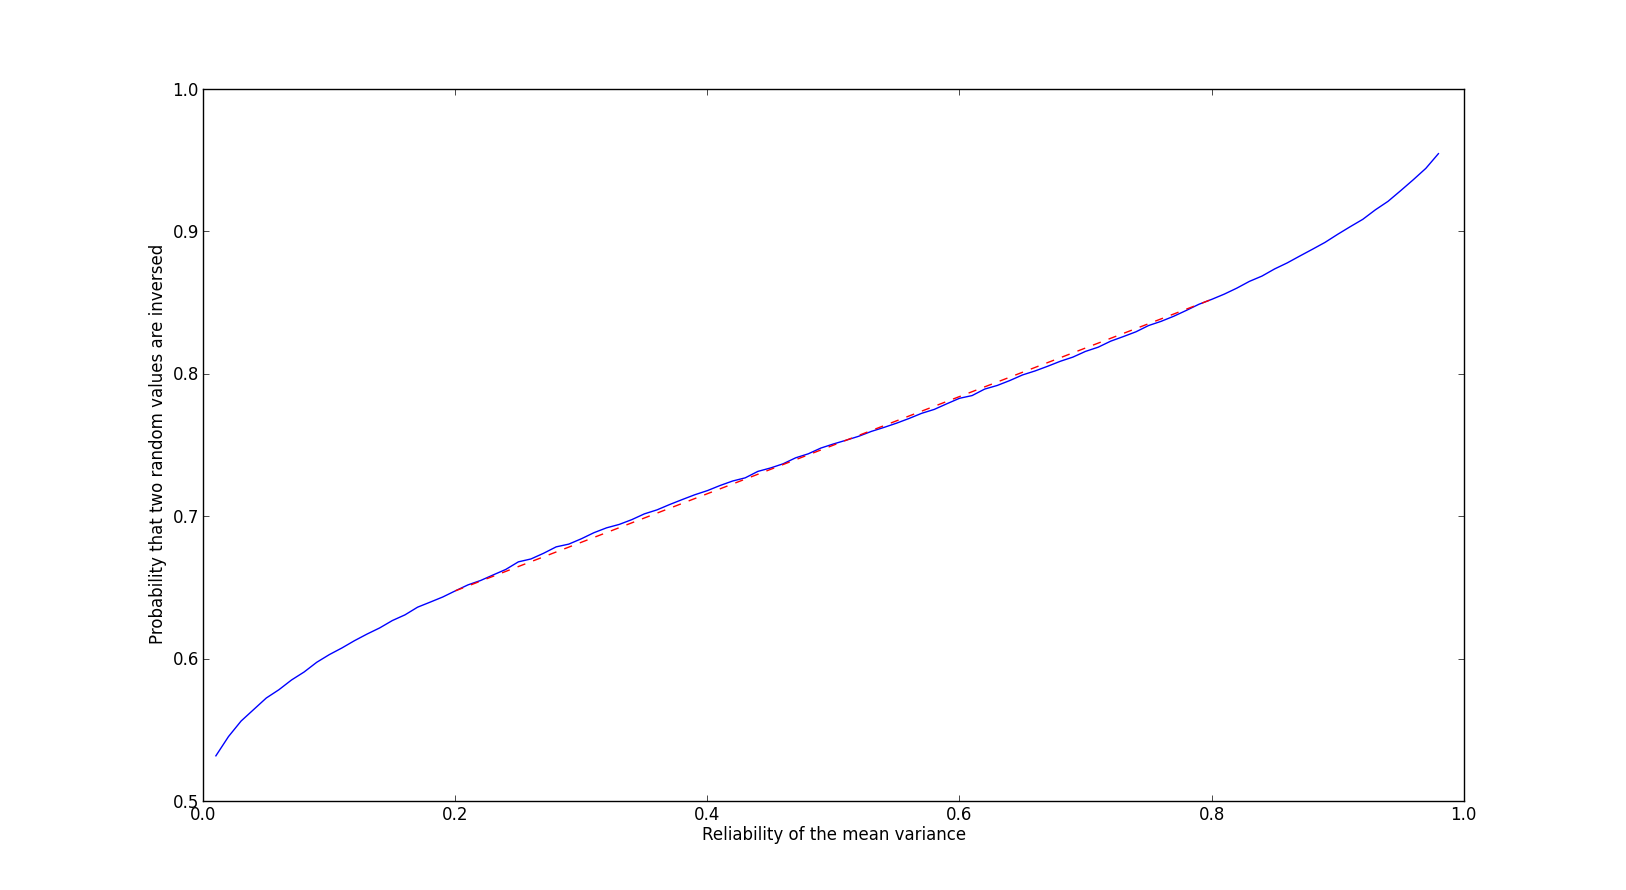
\includegraphics[width=\textwidth]{images/reliVSprob2.png}
\caption{Relation between reliability and percentage of correctly distinguished parameters}
\label{fig:reli}
\end{figure}

When considering the consistency of parameters, a good way to look at them is distinguishability. For example, if we were to look at every possible pair of parameters, in how many cases would the one that is seemingly largest, actually be the largest? The reliability over the average variance of a parameter type is directly related to this measure (see figure \ref{fig:reli})

\subsection{Domains}
\label{sec:domain}
In generating the data there are many other factors that might play a role in the performance of the models. Among those factors are the values that the parameters will be given, the distribution of knowledge components over the items, the ratio of students to items etc. As indicated in section \ref{sec:RQ} these factors are not explored methodically and extensively, but rather a few different datasets are used to represent some of the variation naturally found in this kind of data. The different datasets and some of the characteristics are described in this section.

\subsubsection{Bridge to Algebra}
The first data-set is one of the datasets used in the 2010 KDD cup on education data mining. The data is from Carnegie Learnings' Cognitive Tutor Software meant for high school-students aged 15-18. \cite{ct} provides an overview of some of the features of this program. The data was obtained from the Bridge to Algebra course during the school year 2006-2007 \cite{bridge}. 

\subsubsection{Algebra I}
This dataset was also provided in the 2010 KDD cup. The data is also obtained from Carnegie Learnings' Cognitive Tutor Software, but from the Algebra I course during the school year 2005-2006 \cite{algebra}

\subsection{Assistment}
This dataset is quite different from the other two as it is taken from a web-based ITS named Assistment whose details and development story can be found in \cite{razzaq}. The data is from 12 to 14 year old students and was used in \cite{ktpfa} which was discussed in section \ref{sec:RW}. The data does not only contain data from usage of the ITS but also data from a pre-test.
\subsection{Data cleaning}
\label{sec:cleaning}
Splitting the data may exacerbate some of the issues that can be encountered in fitting the model. One example is when all questions associated with a student or a KC are answered correctly or incorrectly. This makes the fitting algorithm want to assign infinite values to parameters. Another problem is when for a KC there is such a limited number of questions answered that learning rates cannot be estimated.

To prevent these issues the following steps are taken. On the whole dataset, students that answer all questions correctly or incorrectly are removed. In every split KC's for which every question is answered correctly or incorrectly is not taken into account for that split. Additionally if for a KC there is less than two questions answered correctly or incorrectly that KC is not taken into account for that split. This means that this KC is removed from the items and any item that no longer contains a KC is dropped from the data. It is assumed that this does not cause students to now have answered all questions correctly or incorrectly, but this assumption will be checked during the experiments to be certain.

\subsection{KC Experiment}
\subsubsection{The Experiment}
In detail the experiment for KC parameters consists of the following steps per model:
\begin{enumerate}
\item Clean the data by removing students according to section \ref{sec:cleaning}
\item Split the data in a increasing number of parts. Then for each part:
\begin{enumerate}
\item Clean the data by removing KCs according to section \ref{sec:cleaning}
\item Train the model and determine the variance for every parameter type
\item Determine performance on the test-set for that split
\item Determine the inherent variance through the Fisher matrix and through simulation
\item Normalize the found variances with the variances per parameter type found above
\end{enumerate}
\item Determine the variance per parameter over all the splits
\item Normalize the found variances with the average of variances per parameter type found above
\end{enumerate}

\subsubsection{Representing the Results}
Dit is een voorstel voor het representeren van de resultaten. Feedback, ideeen of suggesties worden erg gewaardeerd.
For every split into a number of parts and every model the following will be represented:
\begin{enumerate}
\item The average reliability for each parametertype (both inherent and observed \todo{ preferably the reliability of the difference between the two as well, even though that has not worked too well in the testrun I have shown, although I'm less than 90\% sure I did not make a mistake})
\item The average accuracy and normalized log likelihood
\item Histograms that display the reliabilities of the different parameters. Outliers can now be easily spotted.
\end{enumerate}
\todo{I'd also like to see to what extent inherent and total variance are related over the different splittings and models, as well as relations with accuracy and normalized log likelihood. correlation or spearmans R are two options I'm considering}

\section{results}
Kendall
A few observations on the basis of the figures below. Foremost is the observation that the inherent variance is sometimes higher than the actual observed variance. A possible conclusion might be that reality is not quite as stochastic as the model: you either know a knowledge component or you don't and there is far less of a chance of answering correctly when you don't know an answer or vice versa. The question what part of the variance is due to internal variance is not useful as sometimes the variance is above and sometimes below the variance that is observed. This internal variance might still be useful though as it is rather correlated to the total variance, especially at lower values. (see the figure below)

As expected the variance is less as more data is available although the variance seems to decrease less as data is increased. Also quite obvious is that the learning parameters have far higher variances than the beta parameter. Interestingly adding an additional parameter does not substantially change the variance of the beta parameter.



\begin{figure}
\centering
\subfloat[AFM model on algebra05\_06 dataset]{
  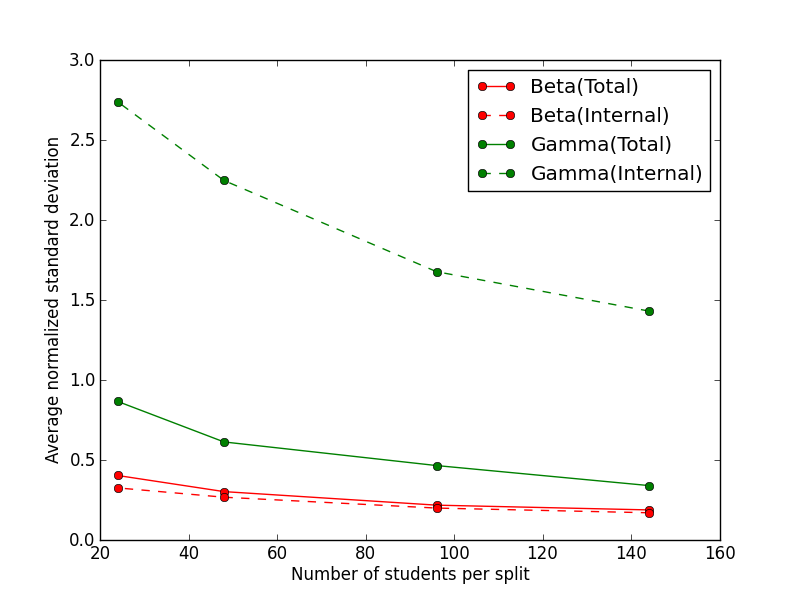
\includegraphics[width=65mm]{images/basicafm.png}
}
\subfloat[PFA model on algebra05\_06 dataset ]{
  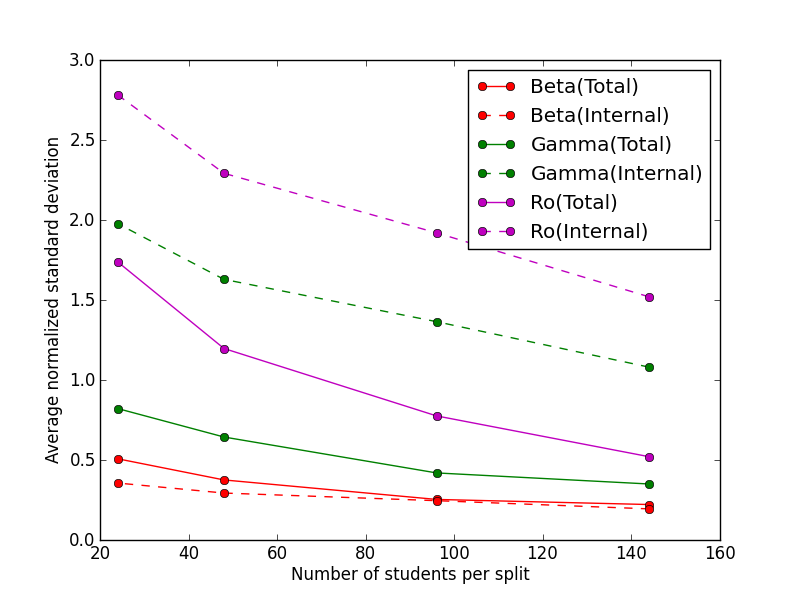
\includegraphics[width=65mm]{images/basicpfa.png}
}
\hspace{0mm}
\subfloat[AFM model on bridgetoAlgebra06\_07 dataset]{
  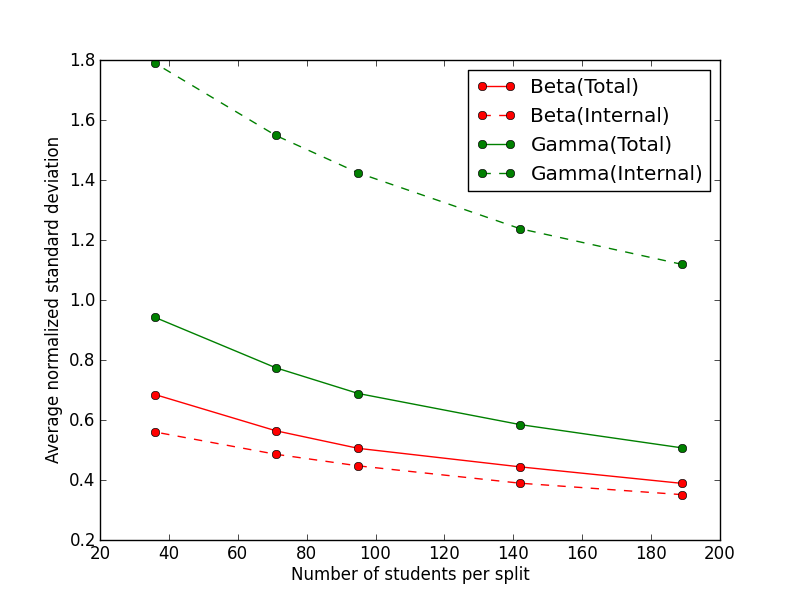
\includegraphics[width=65mm]{images/bridgeafm.png}
}
\subfloat[PFA model on bridgetoAlgebra06\_07 dataset]{
  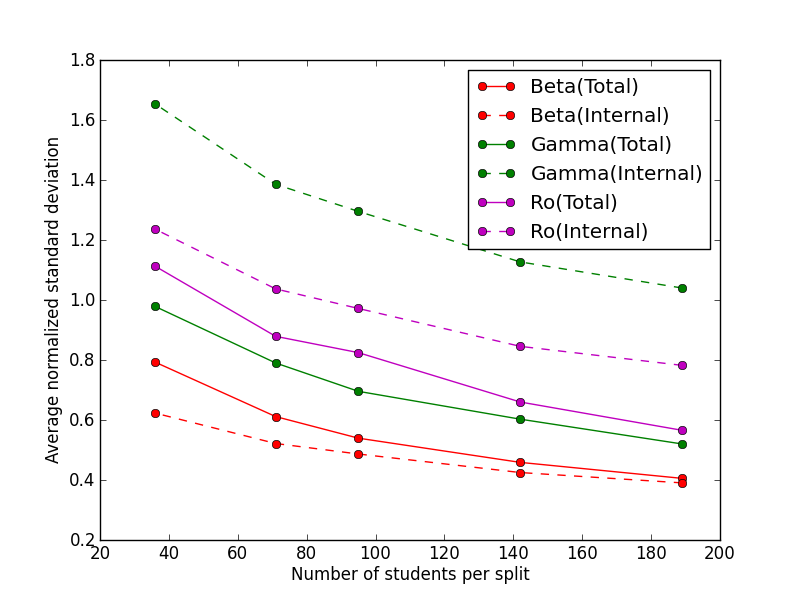
\includegraphics[width=65mm]{images/bridgepfa.png}
}
\hspace{0mm}
\subfloat[AFM model on assistmentGong dataset]{   % ???
  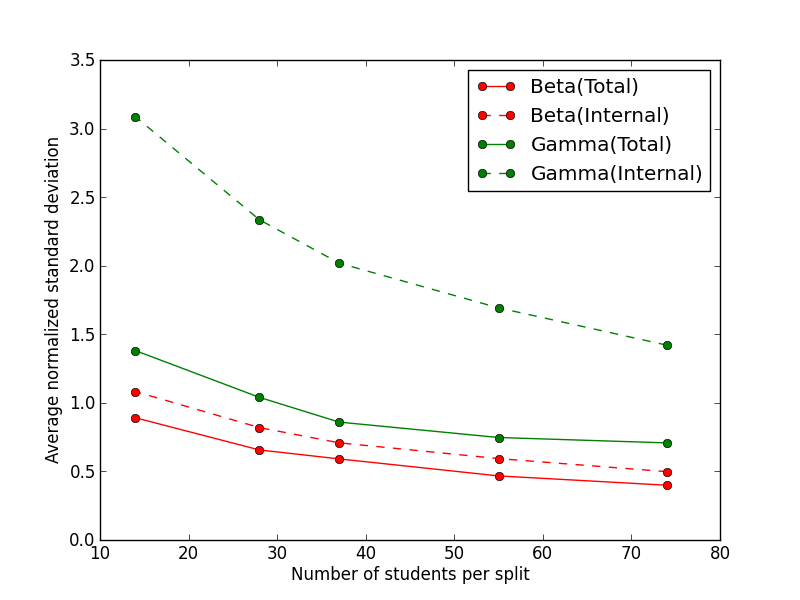
\includegraphics[width=65mm]{images/gongafm.png}
}
\subfloat[PFA model on assistmentGong dataset]{
  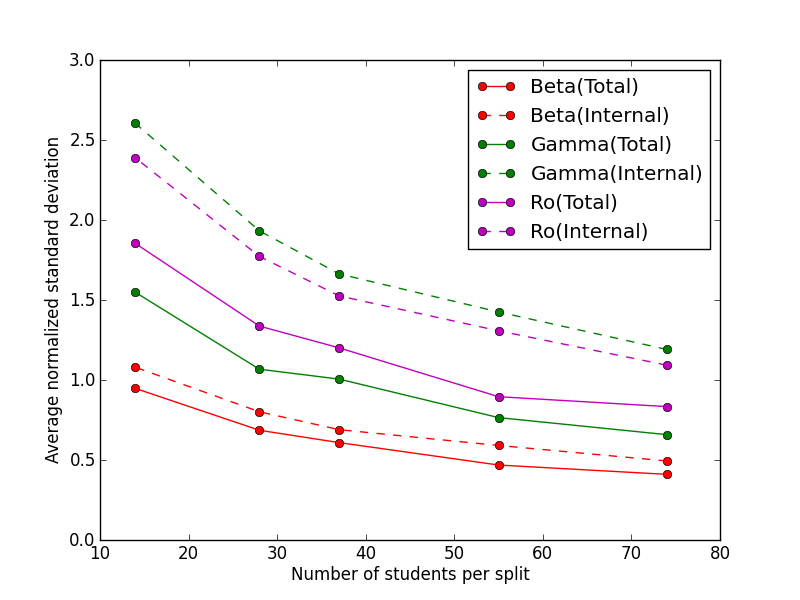
\includegraphics[width=65mm]{images/gongpfa.png}
}
\caption{}
\end{figure}
\begin{figure}
\centering
\subfloat[AFM model, beta parameter]{
  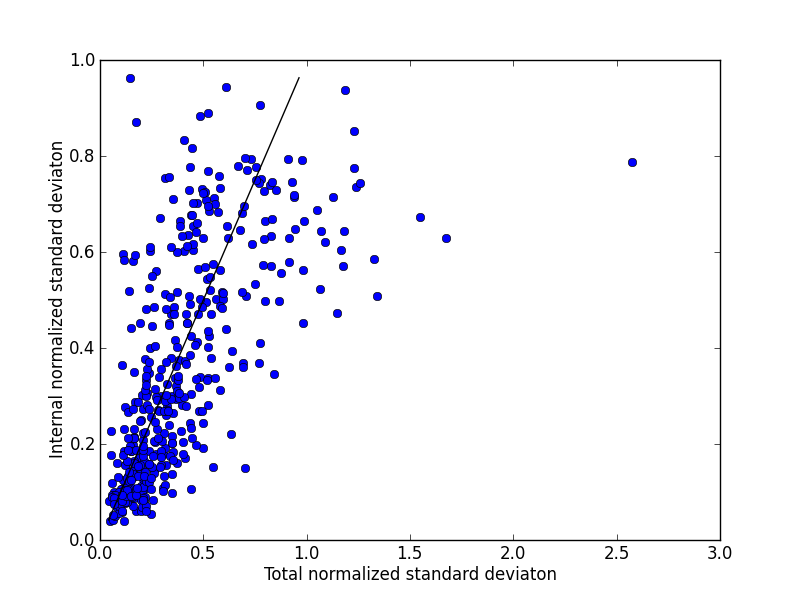
\includegraphics[width=65mm]{images/afm6in_tot_varbeta.png}
}
\subfloat[PFA model, gamma parameter ]{
  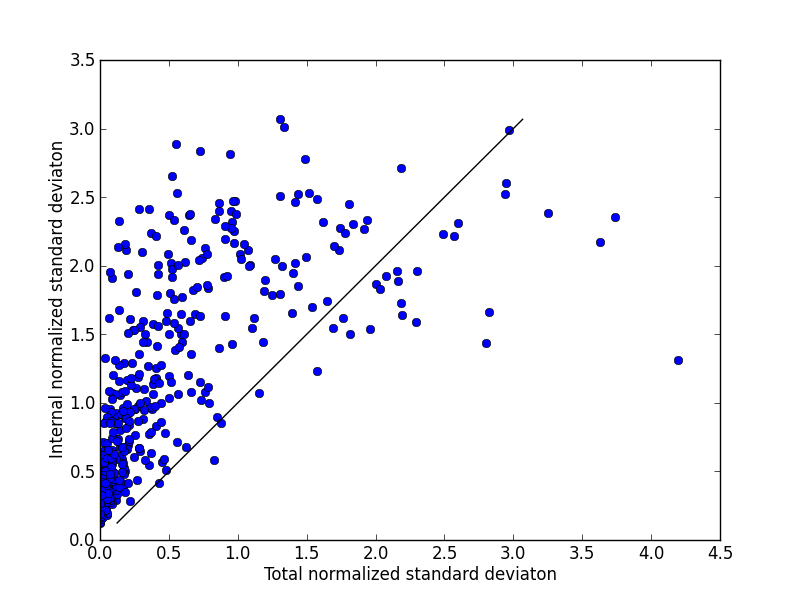
\includegraphics[width=65mm]{images/afm6in_tot_vargamma.png}
}
\hspace{0mm}
\subfloat[PFA model, beta parameter]{
  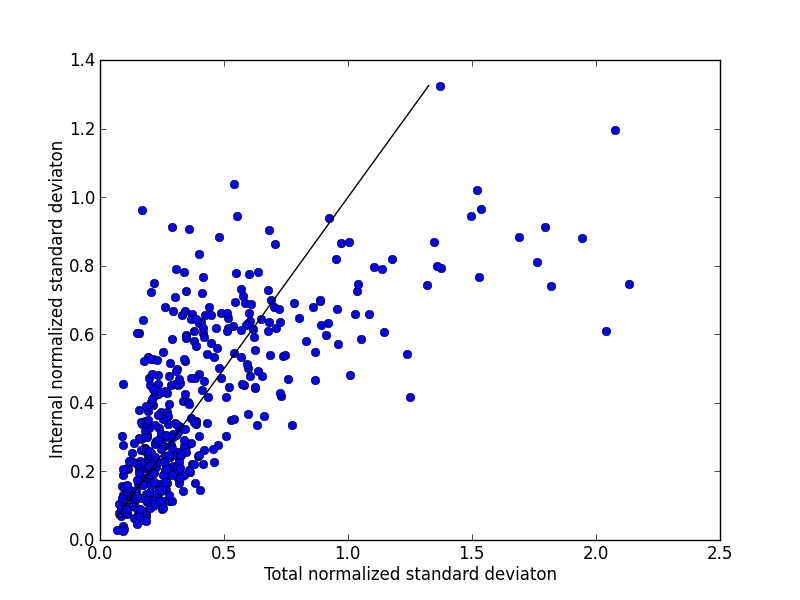
\includegraphics[width=65mm]{images/pfa6in_tot_varbeta.png}
}
\subfloat[PFA model, gamma parameter]{
  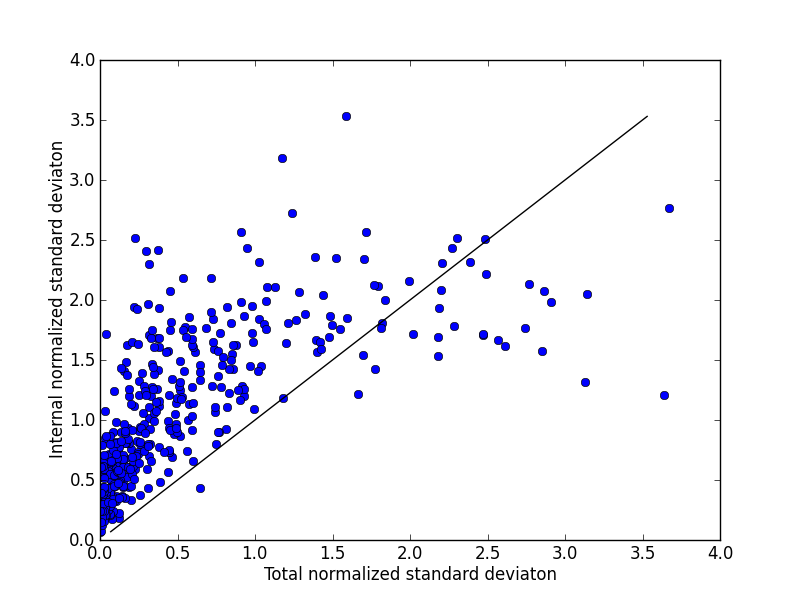
\includegraphics[width=65mm]{images/pfa6in_tot_vargamma.png}
}
\hspace{0mm}
\subfloat[PFA model, ro parameter]{   % ???
  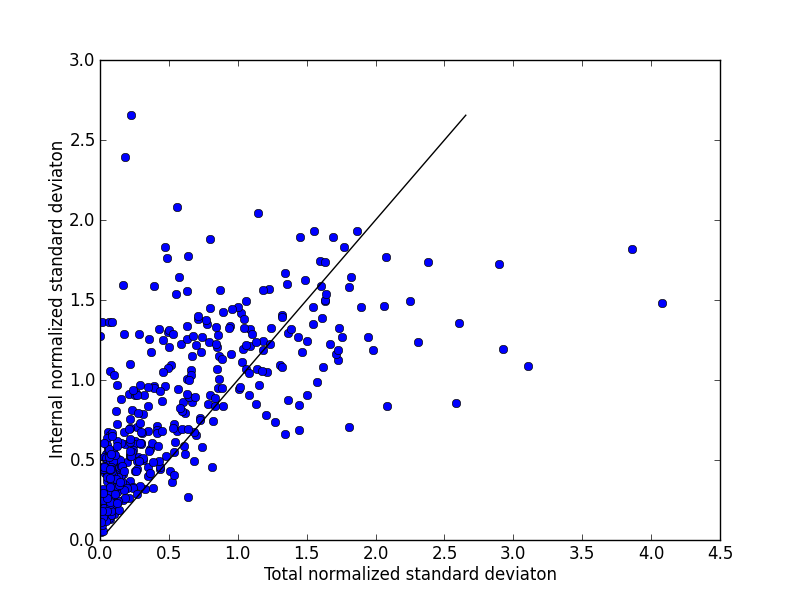
\includegraphics[width=65mm]{images/pfa6in_tot_varro.png}
}

\caption{Standard deviations on the values of individual parameters on the bridgetoAlgebra06\_07 dataset}
\end{figure}
\newpage
\todo{
\section{Things to add and change}
\begin{itemize}
\item Describe terms and use those consistently!
\item implement and describe the adapted A' approach
\item related work is a bit out of place as it is not very intelligible without information given later. Maybe move it to the end, or rather integrate it with other stuff?
\item Describe the datasets and add some extra info on what the datasets look like?
\item Investigate some of the outliers? 
\end{itemize}
}
\bibliographystyle{alpha}   % this means that the order of references
			    % is determined by the order in which the
			    % \cite and \nocite commands appear
\bibliography{litlist}
\newpage
\appendix
\section{Implementation and Mathematical argumentation}
The AFM and PFA model are relatively straightforward in their data representation and implementation. For these models $x$ in formula \ref{eq:logistic} is linear in the parameters, which means that standard logistic regression can be applied. In this appendix first the way the data is represented is described followed by a proof that logistic regression indeed finds the parameter values where the likelihood of the data is highest. 
\subsection{Data Representation}
For logistic regression the data is represented in a matrix $\Phi$ such that $\Phi w$ is equal to a vector of each value of $x$ in formula \ref{eq:logistic}, where $w$ is a column vector of the parameter values. 
In this matrix the rows represent data points while the columns represent what the parameters should be multiplied with. The dimensions of the matrix are thus equal to the number of data points by the number of parameters.

In the formulas for AFM (formula \ref{eq:afm}) and PFA (formula \ref{eq:pfa}) $x$ consists of a sum where every part contains exactly one parameter. This makes construction of $\Phi$ straightforward: in each row (thus for every data point) a 1 is placed for every present parameter that stands isolated (this goes for $\theta$ and $\beta$) and for the others ($\eta$,$\gamma$ and $\rho$) the right value for that data point is inserted (a non-negative integer). Any parameter not used for that specific datapoint will have a value of 0.

\subsection{Workings of Logistic Regression}
Logistic regression estimates the values of the parameters that maximize the likelihood of the data given the model. The likelihood of the data is equal to $\prod_{d \in D} P_{d}^{t_d}  (1- P_{d})^{1-t_d} $
\pagebreak 
\section{Glossary}
\todo{
Making a start with using terms consistently, plus I generally feel that a glossary would have helped me greatly in understanding papers etc.}
\begin{description}
  \item[Item] A problem (step) in the ITS to which a single answer can be given
  \item[Knowledge Component] A skill, piece of knowledge etc. that is associated with one or more items and in which students can have a level of competence
  \item[Question] An instance of an item
  \item[Skill] Level of an instance of a knowledge component for a particular student
\end{description}

\end{document}
